\documentclass{article}
\usepackage[utf8]{inputenc}
\usepackage{geometry}
 \geometry{
 a3paper}
\usepackage{tikz}
\usetikzlibrary{mindmap,backgrounds,calc} % LATEX and plain TEX
\title{Updated Skill Trees}
\author{xuyuanyuan102888 }
\date{December 2024}

\begin{document}

% Tree 1: Programming Languages & Frameworks (Blue theme)
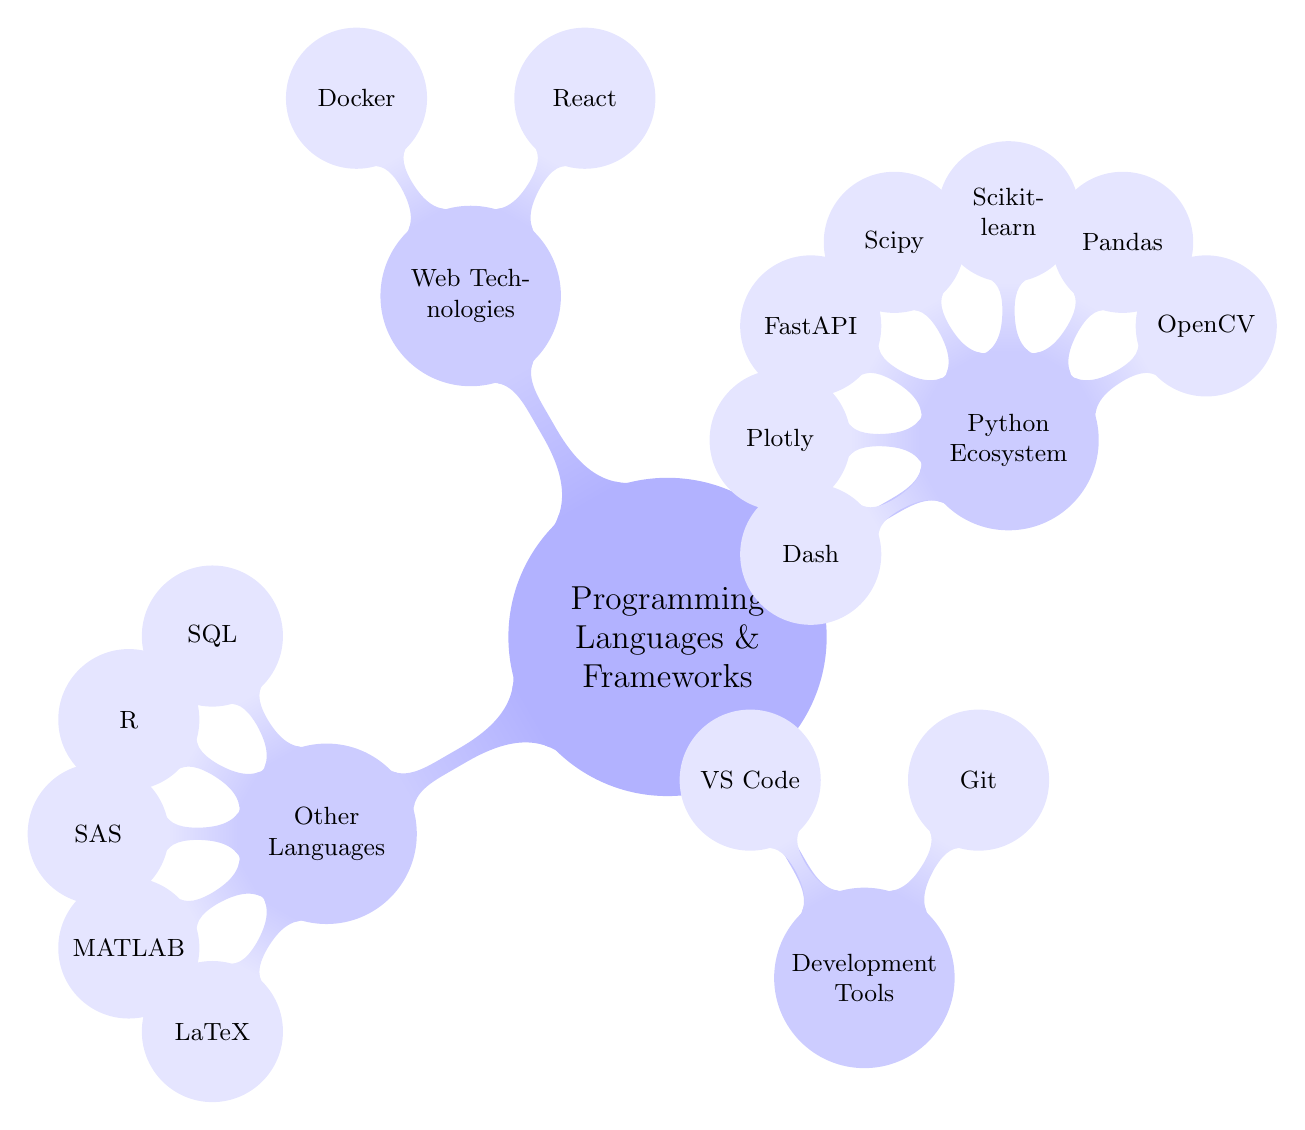
\begin{tikzpicture}
    [mindmap,
    concept color=blue!30,
    every node/.style ={concept},
    every extra concept/.style={
        text = black,
        concept color = blue!10}
    ]
    \node (root1) [concept color = blue!30] {Programming Languages \& Frameworks} 
        child [grow = 30, concept color = blue!20] {
            node {Python Ecosystem}
                child [grow = 30, font=\small, concept color = blue!10] {node {OpenCV}}
                child [grow = 60, font=\small, concept color = blue!10] {node {Pandas}}
                child [grow = 90, font=\small, concept color = blue!10] {node {Scikit-learn}}
                child [grow = 120, font=\small, concept color = blue!10] {node {Scipy}}
                child [grow = 150, font=\small, concept color = blue!10] {node {FastAPI}}
                child [grow = 180, font=\small, concept color = blue!10] {node {Plotly}}
                child [grow = 210, font=\small, concept color = blue!10] {node {Dash}}
        }
        child [grow = 120, concept color = blue!20] {
            node {Web Technologies}
                child [grow = 60, font=\small, concept color = blue!10] {node {React}}
                child [grow = 120, font=\small, concept color = blue!10] {node {Docker}}
        }
        child [grow = 210, concept color = blue!20] {
            node {Other Languages}
                child [grow = 120, font=\small, concept color = blue!10] {node {SQL}}
                child [grow = 150, font=\small, concept color = blue!10] {node {R}}
                child [grow = 180, font=\small, concept color = blue!10] {node {SAS}}
                child [grow = 210, font=\small, concept color = blue!10] {node {MATLAB}}
                child [grow = 240, font=\small, concept color = blue!10] {node {LaTeX}}
        }
        child [grow = 300, concept color = blue!20] {
            node {Development Tools}
                child [grow = 60, font=\small, concept color = blue!10] {node {Git}}
                child [grow = 120, font=\small, concept color = blue!10] {node {VS Code}}
        }
    ;
\end{tikzpicture}

\vspace{2cm}

% Tree 2: Cloud & Infrastructure (Green theme)
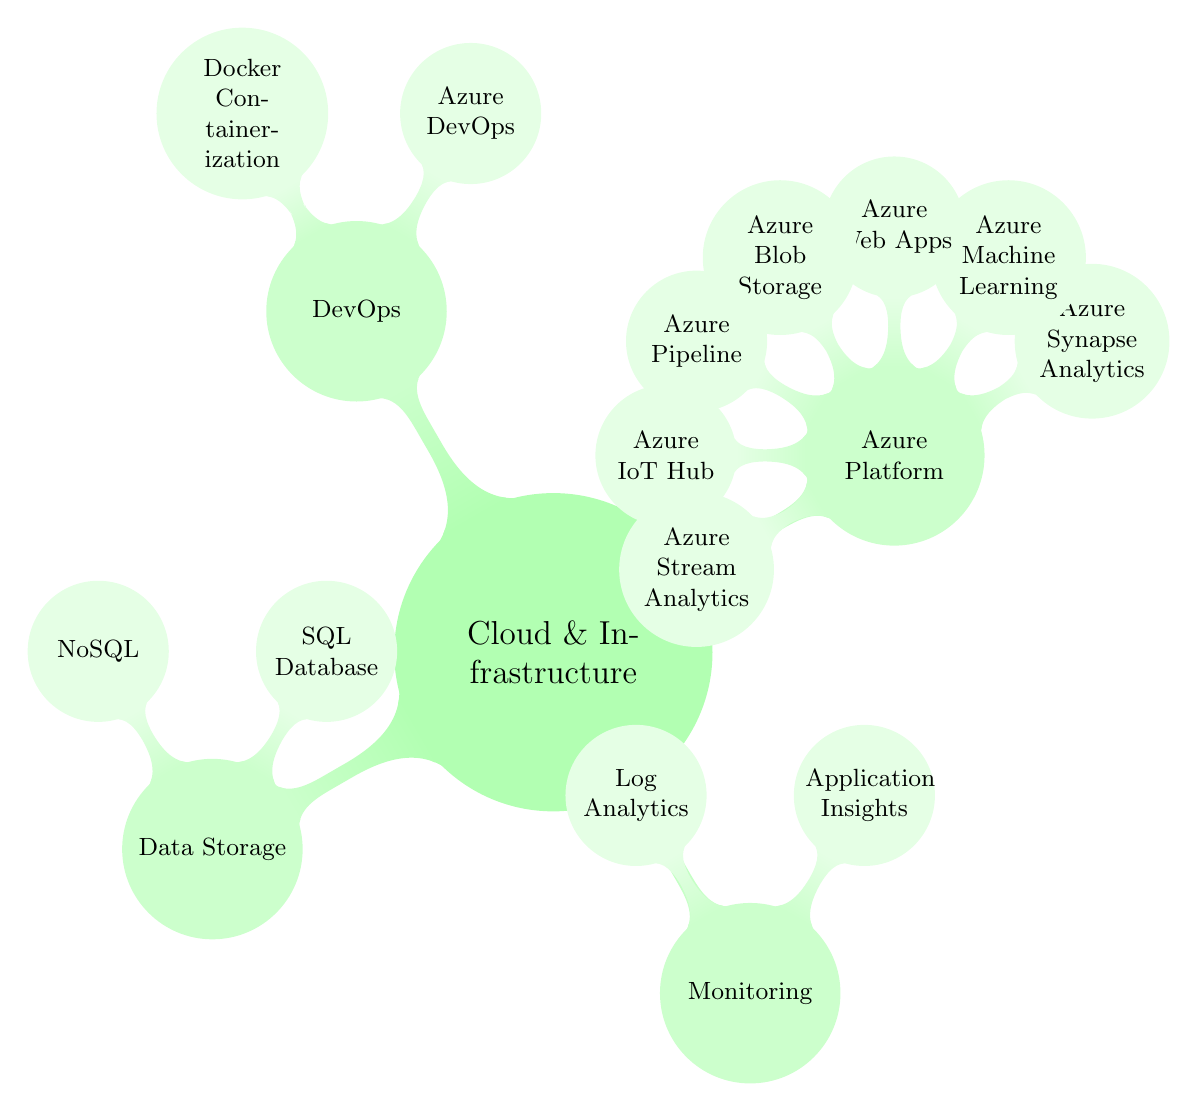
\begin{tikzpicture}
    [mindmap,
    concept color=green!30,
    every node/.style ={concept},
    every extra concept/.style={
        text = black,
        concept color = green!10}
    ]
    \node (root2) [concept color = green!30] {Cloud \& Infrastructure} 
        child [grow = 30, concept color = green!20] {
            node {Azure Platform}
                child [grow = 30, font=\small, concept color = green!10] {node {Azure Synapse Analytics}}
                child [grow = 60, font=\small, concept color = green!10] {node {Azure Machine Learning}}
                child [grow = 90, font=\small, concept color = green!10] {node {Azure Web Apps}}
                child [grow = 120, font=\small, concept color = green!10] {node {Azure Blob Storage}}
                child [grow = 150, font=\small, concept color = green!10] {node {Azure Pipeline}}
                child [grow = 180, font=\small, concept color = green!10] {node {Azure IoT Hub}}
                child [grow = 210, font=\small, concept color = green!10] {node {Azure Stream Analytics}}
        }
        child [grow = 120, concept color = green!20] {
            node {DevOps}
                child [grow = 60, font=\small, concept color = green!10] {node {Azure DevOps}}
                child [grow = 120, font=\small, concept color = green!10] {node {Docker Containerization}}
        }
        child [grow = 210, concept color = green!20] {
            node {Data Storage}
                child [grow = 60, font=\small, concept color = green!10] {node {SQL Database}}
                child [grow = 120, font=\small, concept color = green!10] {node {NoSQL}}
        }
        child [grow = 300, concept color = green!20] {
            node {Monitoring}
                child [grow = 60, font=\small, concept color = green!10] {node {Application Insights}}
                child [grow = 120, font=\small, concept color = green!10] {node {Log Analytics}}
        }
    ;
\end{tikzpicture}

\vspace{2cm}

% Tree 3: AI & Machine Learning (Purple theme)
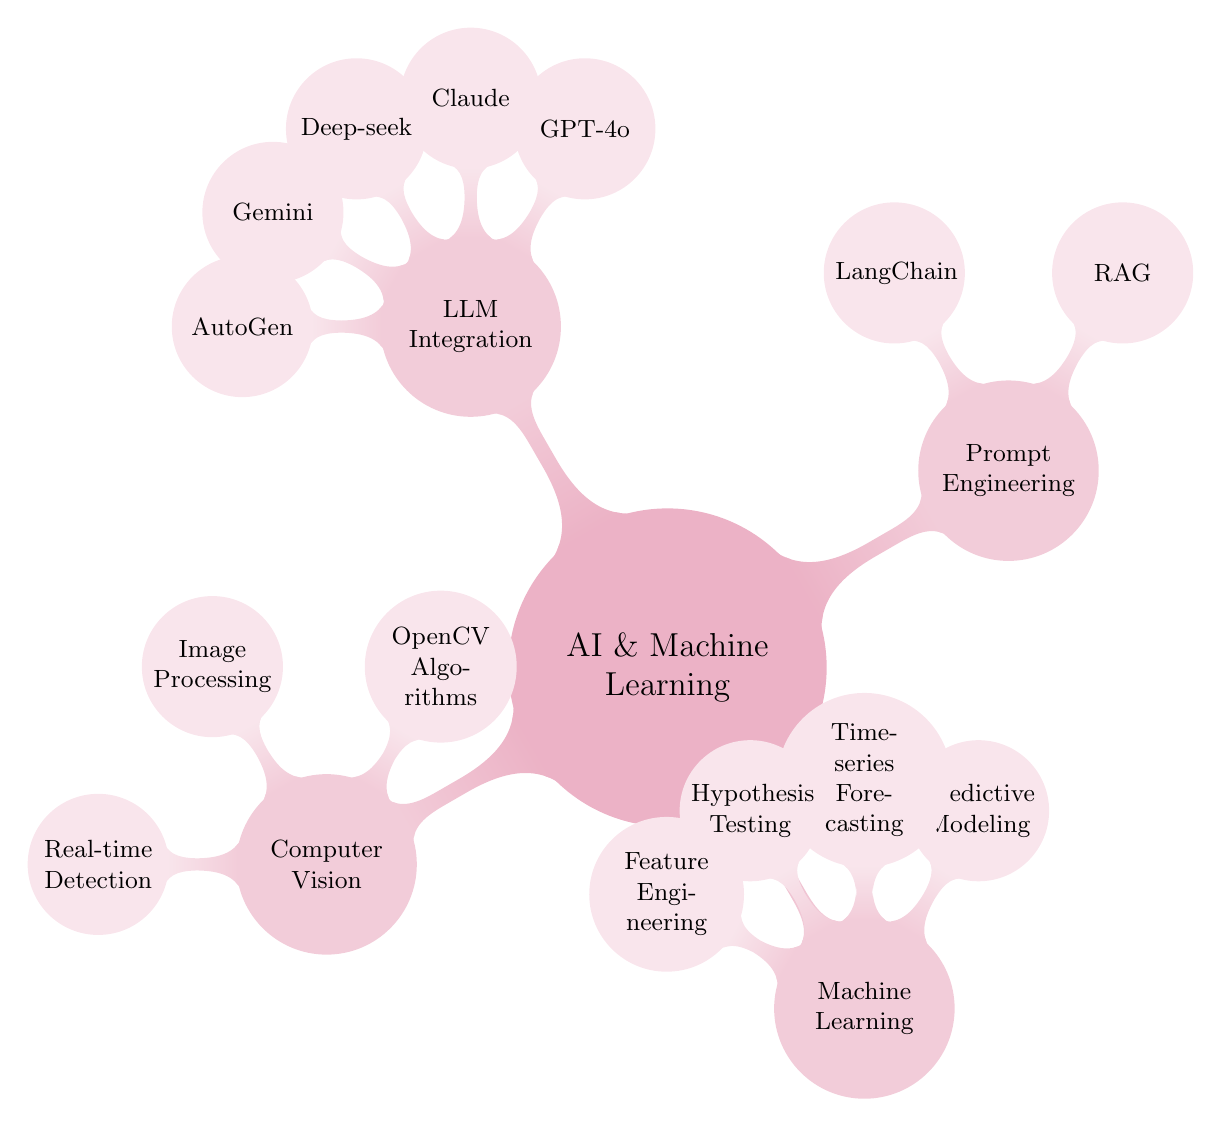
\begin{tikzpicture}
    [mindmap,
    concept color=purple!30,
    every node/.style ={concept},
    every extra concept/.style={
        text = black,
        concept color = purple!10}
    ]
    \node (root3) [concept color = purple!30] {AI \& Machine Learning} 
        child [grow = 30, concept color = purple!20] {
            node {Prompt Engineering}
                child [grow = 60, font=\small, concept color = purple!10] {node {RAG}}
                child [grow = 120, font=\small, concept color = purple!10] {node {LangChain}}
        }
        child [grow = 120, concept color = purple!20] {
            node {LLM Integration}
                child [grow = 60, font=\small, concept color = purple!10] {node {GPT-4o}}
                child [grow = 90, font=\small, concept color = purple!10] {node {Claude}}
                child [grow = 120, font=\small, concept color = purple!10] {node {Deep-seek}}
                child [grow = 150, font=\small, concept color = purple!10] {node {Gemini}}
                child [grow = 180, font=\small, concept color = purple!10] {node {AutoGen}}
        }
        child [grow = 210, concept color = purple!20] {
            node {Computer Vision}
                child [grow = 60, font=\small, concept color = purple!10] {node {OpenCV Algorithms}}
                child [grow = 120, font=\small, concept color = purple!10] {node {Image Processing}}
                child [grow = 180, font=\small, concept color = purple!10] {node {Real-time Detection}}
        }
        child [grow = 300, concept color = purple!20] {
            node {Machine Learning}
                child [grow = 60, font=\small, concept color = purple!10] {node {Predictive Modeling}}
                child [grow = 90, font=\small, concept color = purple!10] {node {Time-series Forecasting}}
                child [grow = 120, font=\small, concept color = purple!10] {node {Hypothesis Testing}}
                child [grow = 150, font=\small, concept color = purple!10] {node {Feature Engineering}}
        }
    ;
\end{tikzpicture}

\vspace{2cm}

% Tree 4: Data Analytics & Visualization (Orange theme)
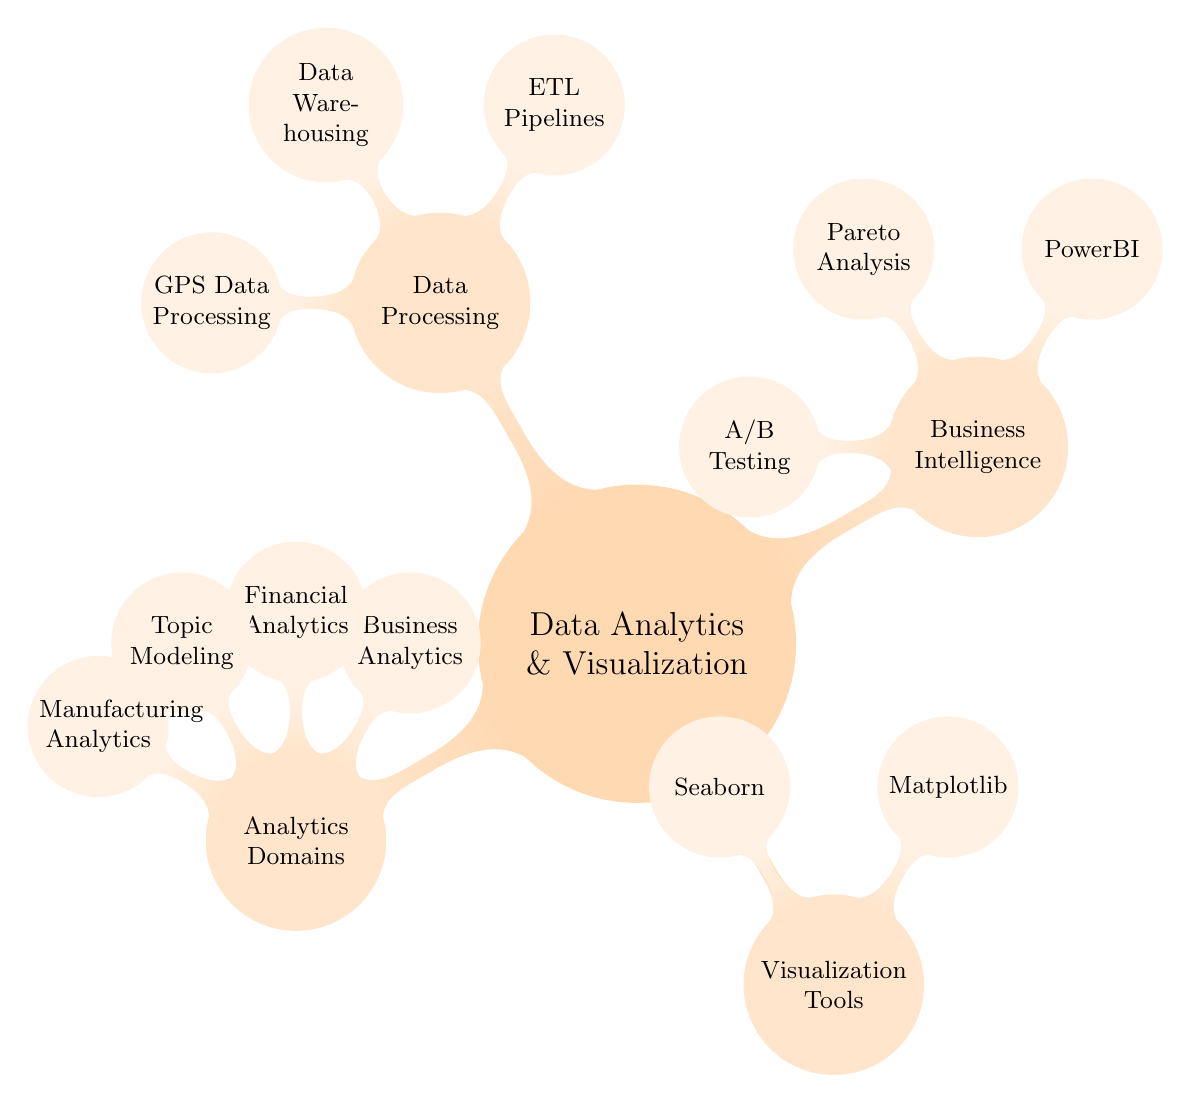
\begin{tikzpicture}
    [mindmap,
    concept color=orange!30,
    every node/.style ={concept},
    every extra concept/.style={
        text = black,
        concept color = orange!10}
    ]
    \node (root4) [concept color = orange!30] {Data Analytics \& Visualization} 
        child [grow = 30, concept color = orange!20] {
            node {Business Intelligence}
                child [grow = 60, font=\small, concept color = orange!10] {node {PowerBI}}
                child [grow = 120, font=\small, concept color = orange!10] {node {Pareto Analysis}}
                child [grow = 180, font=\small, concept color = orange!10] {node {A/B Testing}}
        }
        child [grow = 120, concept color = orange!20] {
            node {Data Processing}
                child [grow = 60, font=\small, concept color = orange!10] {node {ETL Pipelines}}
                child [grow = 120, font=\small, concept color = orange!10] {node {Data Warehousing}}
                child [grow = 180, font=\small, concept color = orange!10] {node {GPS Data Processing}}
        }
        child [grow = 210, concept color = orange!20] {
            node {Analytics Domains}
                child [grow = 60, font=\small, concept color = orange!10] {node {Business Analytics}}
                child [grow = 90, font=\small, concept color = orange!10] {node {Financial Analytics}}
                child [grow = 120, font=\small, concept color = orange!10] {node {Topic Modeling}}
                child [grow = 150, font=\small, concept color = orange!10] {node {Manufacturing Analytics}}
        }
        child [grow = 300, concept color = orange!20] {
            node {Visualization Tools}
                child [grow = 60, font=\small, concept color = orange!10] {node {Matplotlib}}
                child [grow = 120, font=\small, concept color = orange!10] {node {Seaborn}}
        }
    ;
\end{tikzpicture}

\vspace{2cm}

% Tree 5: Industrial Applications (Teal theme)
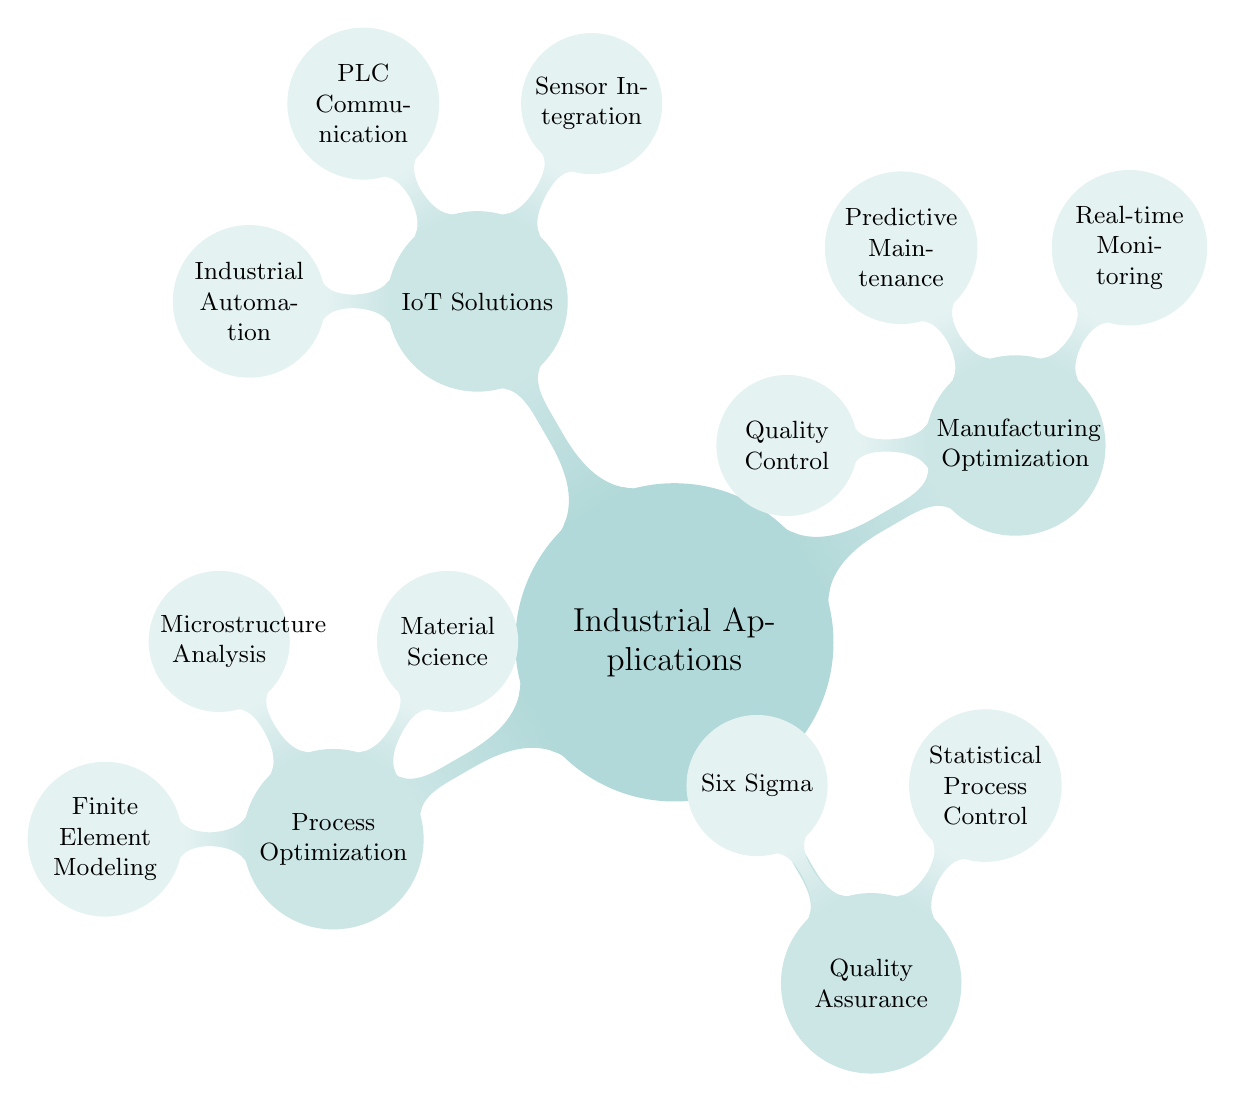
\begin{tikzpicture}
    [mindmap,
    concept color=teal!30,
    every node/.style ={concept},
    every extra concept/.style={
        text = black,
        concept color = teal!10}
    ]
    \node (root5) [concept color = teal!30] {Industrial Applications} 
        child [grow = 30, concept color = teal!20] {
            node {Manufacturing Optimization}
                child [grow = 60, font=\small, concept color = teal!10] {node {Real-time Monitoring}}
                child [grow = 120, font=\small, concept color = teal!10] {node {Predictive Maintenance}}
                child [grow = 180, font=\small, concept color = teal!10] {node {Quality Control}}
        }
        child [grow = 120, concept color = teal!20] {
            node {IoT Solutions}
                child [grow = 60, font=\small, concept color = teal!10] {node {Sensor Integration}}
                child [grow = 120, font=\small, concept color = teal!10] {node {PLC Communication}}
                child [grow = 180, font=\small, concept color = teal!10] {node {Industrial Automation}}
        }
        child [grow = 210, concept color = teal!20] {
            node {Process Optimization}
                child [grow = 60, font=\small, concept color = teal!10] {node {Material Science}}
                child [grow = 120, font=\small, concept color = teal!10] {node {Microstructure Analysis}}
                child [grow = 180, font=\small, concept color = teal!10] {node {Finite Element Modeling}}
        }
        child [grow = 300, concept color = teal!20] {
            node {Quality Assurance}
                child [grow = 60, font=\small, concept color = teal!10] {node {Statistical Process Control}}
                child [grow = 120, font=\small, concept color = teal!10] {node {Six Sigma}}
        }
    ;
\end{tikzpicture}

\end{document}
